\section{Method} \label{sec:method}


\subsection{Analysis on Compact Convolutional Neural Network}

\begin{figure}[htbp]
\centerline{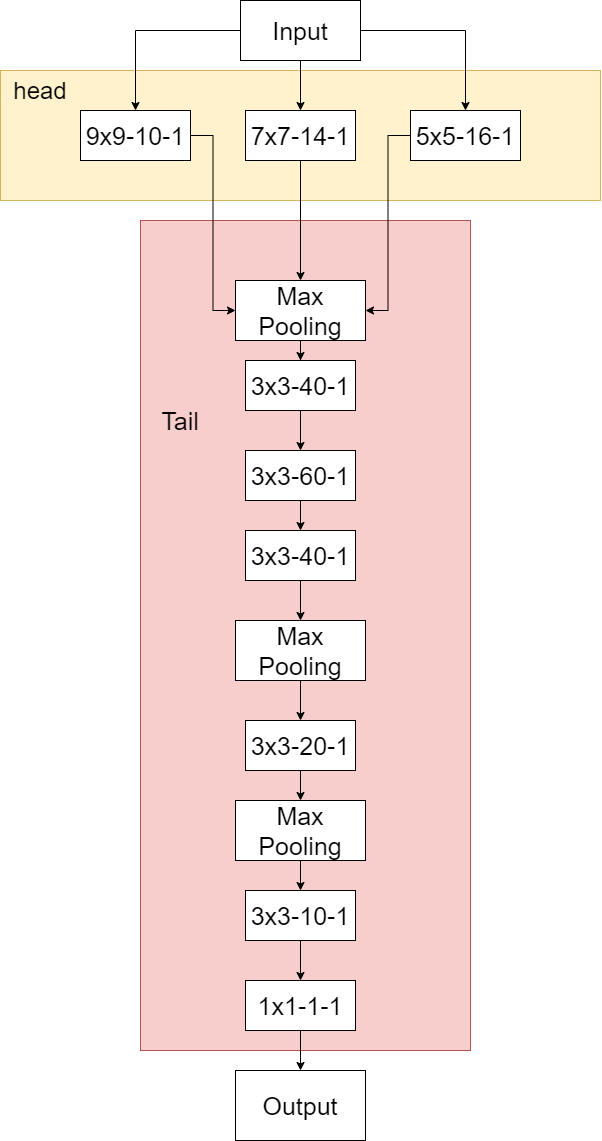
\includegraphics[width=0.4\textwidth]{Picture/proposed/ccnn_original_fix1.png}}
\caption{C-CNN architecture in our re-implementation}
\label{fig:ccnn}
\end{figure}



Despite their performance, state-of-the-art models are complex. C-CNN is a bargain trade performance for efficiency. Fig.\ref{fig:ccnn} is C-CNN from original works \cite{9053780}. We call three branch convolution layer with different kernel size as the "head", and the rest as the tail. CNN module are remark as (kernel size)-(number of filter)-(dilated rate). 

Despite light-weight, C-CNN \cite{9053780} can tackle the problem of scale variation with its "head", consist of 3 parallel CNN with different kernel size. The early feature fusion after first layer not only reduce model complexity but also avoid problem of redundancy in later layer of MCNN \cite{zhang2016single}, which have bean investigate by Li et al. \cite{li2018csrnet}. 
However, there is still room for improvement, as C-CNN does not provide any mechanism to alleviate background noise.

% we going Dilated and average pooling
\subsection{Dilated Compact Convolutional Neural Network (DCCNN)} 

\begin{figure}[htbp]
\centerline{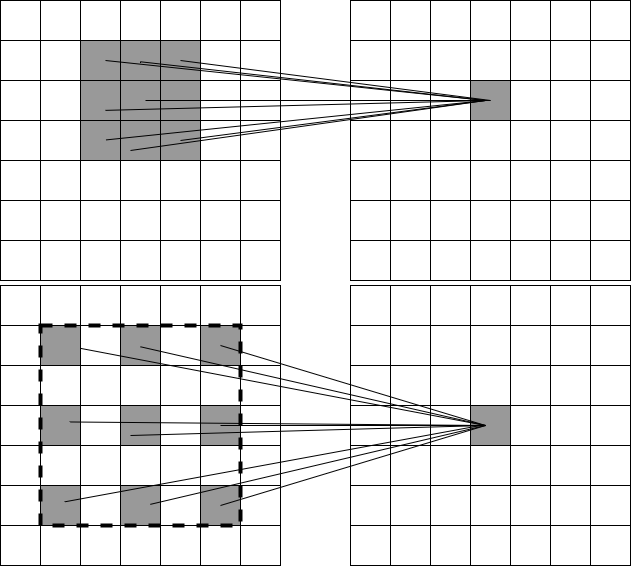
\includegraphics[width=0.4\textwidth]{Picture/example/cnn_vs_dilated_cnn.png}}
\caption{Traditional convolution with dilated rate 1 (top) and dilated convolution with dilated rate 2 (bottom)}
\label{fig:cnn_vs_dilated}
\end{figure}

Dilated convolution with dilated rate n have space n-1 unit between the kernel points. Fig. \ref{fig:cnn_vs_dilated} illustrates dilated convolution with dilated rate 2 (bottom) with traditional convolution, whose dilated rate is 1. Dilated convolution can expand the receptive field of without increase kernel size.

Dilated convolution have been proven to conserved spatial context information  and deliver sharper feature map \cite{li2018csrnet}. We hypothesis Dilated convolution can solve the problem of background noise at low cost. Dilated convolution also been widely use in back-end decoder in recent crowd counting model, such as CSRNet \cite{li2018csrnet}, CAN \cite{liu2019context}, DMCNN \cite{zhang2019crowd}, TEDNet \cite{jiang2019crowd}. Inspired by their success, we replace layer all tradition CNN on second layer with Dilated CNN at dilated rate 2. We replace the second and third max-pooling layer into average-pooling to prevent loss of head count in max function \cite{zhang2019crowd}. 

We apply batch normalization \cite{ioffe2015batch} with trainable affine parameters on each CNN layer, including first multi-scale layers. Follow authors work, we add batch normalization before the nonlinearity, in our case, before ReLU activation \cite{agarap2018deep}. 

Fig. \ref{fig:dccnn} is the implementation of our proposed DCCNN.  We hypothesis that DCCNN becomes more robust to background noise, which yields better performance on medium and sparse crowd scenes. 
% Comparing to C-CNN, our proposed model require slightly increase in computation cost and memory due to:

% \begin{itemize}
%     \item 
% \end{itemize}

% \begin{table}[htbp]
% \caption{Experiment result}

\begin{figure}[htbp]
\centerline{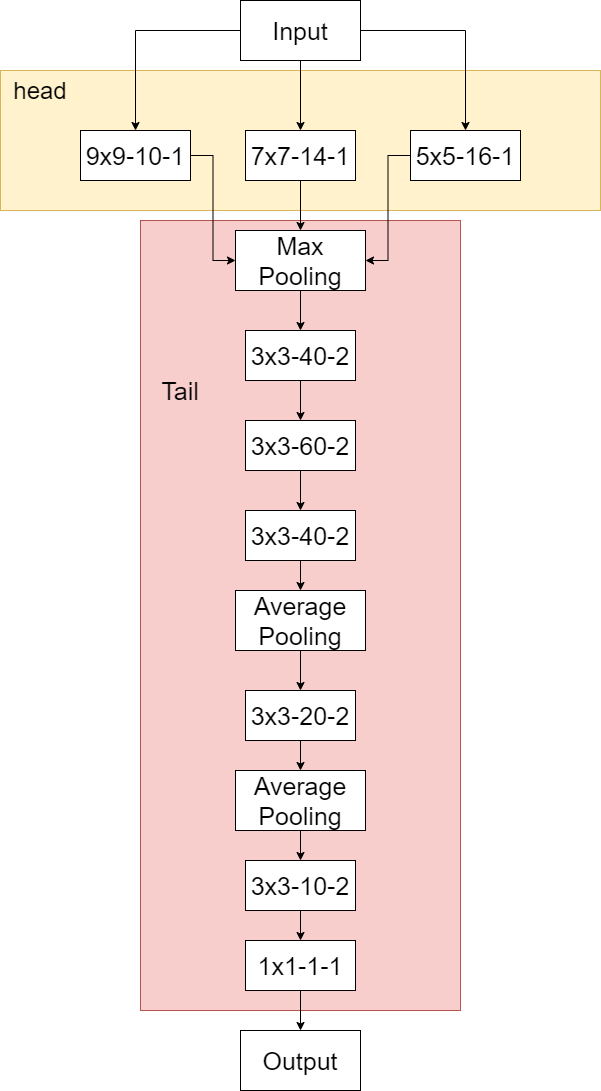
\includegraphics[width=0.4\textwidth]{Picture/proposed/tail13_fix2.png}}
\caption{Our proposed network}
\label{fig:dccnn}
\end{figure}



\subsection{Implementation detail}

\subsubsection{Ground-truth generation} \hfill

For ShanghaiTech Part B dataset, we apply Gaussian kernel, original proposed by Lempitsky, \cite{lempitsky2010learning} with $\sigma = 15$ and truncate Gaussian spread at 3 standard deviations. Truncate Gaussian spread help us prevent noise in ground truth density maps, ensure that label at no-human zone is zero. For each image $I_i$, we define ground truth density function as: 

\begin{equation} \label{eq:densit-function}
\forall p \in I_{i}, \quad F_{i}^{0}(p)=\sum_{P \in \mathbf{P}_{i}} \mathcal{N}\left(p ; P, \sigma^{2} \mathbf{1}_{2 \times 2}\right) 
\end{equation}

Where: 
\begin{itemize}
  \item $p$ is pixel
  \item $\mathbf{P}_{i}$ is set of annotated point of image $i$
\end{itemize}

Total people count in image can be acquired by integral (\ref{eq:densit-function}) over whole density map,

% as equation: 

% \begin{equation} \label{eq:count}
% C(I_i) = \sum_{p \in I_{i}} F_{i}(p)
% \end{equation}



\subsubsection{Training detail} \hfill

 Because density map estimation is a pixel-wise task, exposing the model to the same set of pixels can cause overfitting \cite{marsden2016fully}. To augment ShanghaiTech B dataset, we crop the image into 4 non-overlap patches, each patch we create a copy of its flip over. Each full image can generate 8 training patches. 

We train our model on loss function $L$ composite of Manhattan distance ( $L1$ loss ) and Euclidean distance ($L_2$ loss): 

\begin{equation}L_2(\Theta)=\frac{1}{N} \sum_{i=1}^{N}\left\|Z\left(X_{i} ; \Theta\right)-Z_{i}^{G T}\right\|^{2}\end{equation}

\begin{equation}L_1(\Theta)=\frac{1}{N} \sum_{i=1}^{N}\left\|Z\left(X_{i} ; \Theta\right)-Z_{i}^{G T}\right\|\end{equation}

\begin{equation}
    L(\Theta) = \frac{1}{2}L_1(\Theta) + \frac{1}{2}L_2(\Theta)
\end{equation}

\begin{itemize}
  \item $\Theta$ is set of model parameters
  \item $Z\left(X_{i} ; \Theta\right)$ is predicted density map from image $I_i$
  \item $Z_{i}^{G T}$ is ground truth density map generated from annotated head of image $I_i$
\end{itemize}

 
 We train the model end-to-end with batch size of 40 patches and AdamW optimizer \cite{loshchilov2017decoupled} with learning rate of 0.001 and weight-decay 0.1. The following source code \footnote{https://github.com/ttpro1995/crowd\_counting\_framework} and setting \footnote{train\_script/learnstuff/l1/adamw1\_bigtail13i\_t1\_shb.sh} can reproduce result in approximately 8 hours of training.



%% TODO





